\documentclass[12pt]{article}
\usepackage[utf8]{inputenc}
\usepackage[spanish, es-tabla, es-lcroman, es-noquoting]{babel}
\selectlanguage{spanish} 
\usepackage{graphicx} %package to manage images
\graphicspath{ {./fotos/} } %ruta relativa fotos
\usepackage{enumerate} % enumerados
\usepackage{subfig} %para concatenar imágenes
\usepackage{vmargin} %para los márgenes
\usepackage{listings} %para poner código
\usepackage{amsmath} %para poner matrices
\usepackage{amssymb} %para utilizar algunos símbolos matemáticos
\usepackage{float}

\setpapersize{A4}
\setmargins{2.5cm}       % margen izquierdo
{1.5cm}                        % margen superior
{16.5cm}                      % anchura del texto
{23.42cm}                    % altura del texto
{10pt}                           % altura de los encabezados
{1cm}                           % espacio entre el texto y los encabezados
{0pt}                             % altura del pie de página
{2cm}                           % espacio entre el texto y el pie de página

\title{\textbf{Práctica 3: Programación.\\ Ajuste de Modelos Lineales.}}
\author{José María Borrás Serrano}
\date{}
\begin{document}
\lstset{language=Python}
\lstset{literate=
  {á}{{\'a}}1 {é}{{\'e}}1 {í}{{\'i}}1 {ó}{{\'o}}1 {ú}{{\'u}}1
  {Á}{{\'A}}1 {É}{{\'E}}1 {Í}{{\'I}}1 {Ó}{{\'O}}1 {Ú}{{\'U}}1
  {à}{{\`a}}1 {è}{{\`e}}1 {ì}{{\`i}}1 {ò}{{\`o}}1 {ù}{{\`u}}1
  {À}{{\`A}}1 {È}{{\'E}}1 {Ì}{{\`I}}1 {Ò}{{\`O}}1 {Ù}{{\`U}}1
  {ä}{{\"a}}1 {ë}{{\"e}}1 {ï}{{\"i}}1 {ö}{{\"o}}1 {ü}{{\"u}}1
  {Ä}{{\"A}}1 {Ë}{{\"E}}1 {Ï}{{\"I}}1 {Ö}{{\"O}}1 {Ü}{{\"U}}1
  {â}{{\^a}}1 {ê}{{\^e}}1 {î}{{\^i}}1 {ô}{{\^o}}1 {û}{{\^u}}1
  {Â}{{\^A}}1 {Ê}{{\^E}}1 {Î}{{\^I}}1 {Ô}{{\^O}}1 {Û}{{\^U}}1
  {œ}{{\oe}}1 {Œ}{{\OE}}1 {æ}{{\ae}}1 {Æ}{{\AE}}1 {ß}{{\ss}}1
  {ű}{{\H{u}}}1 {Ű}{{\H{U}}}1 {ő}{{\H{o}}}1 {Ő}{{\H{O}}}1
  {ç}{{\c c}}1 {Ç}{{\c C}}1 {ø}{{\o}}1 {å}{{\r a}}1 {Å}{{\r A}}1
  {€}{{\EUR}}1 {£}{{\pounds}}1
}

\maketitle

\clearpage

\tableofcontents

\clearpage

Nota: la semilla que hemos utilizado en esta pŕactica para todos los procedemientos aleatorios es $19$.

\section{Comprensión del problema a resolver}

En esta práctica vamos a resolver un problema de clasificación y otro de regresión, cada uno asociado a una base de datos distinta.

Las dos bases de datos que tenemos son:\\

-- \textit{Optical Recognition of Handwritten Digits Data Set}

-- \textit{Communities and Crime Data Set}

\subsection{Optical Recognition of Handwritten Digits Data Set}

La base de datos \textit{Optical Recognition of Handwritten Digits Data Set} está compuesta de un conjunto de imágenes de dígitos manuscritos, donde cada imagen se ha escaneado con una resolución 32x32 y siendo cada píxel blanco o negro, luego se ha dividido en bloques que no se solapan de 4x4 y se ha contado el número de píxeles negros en cada bloque. Así, se genera una matriz 8x8 donde cada elemento es un entero en el rango [0, 16]. \\

En la base de datos cada fila representa un dato distinto y cada columna un atributo.
Cada dato tiene 65 atributos, los 64 primeros son atributos numéricos, donde cada atributo es un elemento de la matriz 8x8 que hemos descrito, y el último atributo es categórico e identifica la clase del dato, es decir, es el número que representa al dígito.\\

Se trata de un problema de aprendizaje supervisado ya que estamos trabajando con datos etiquetados y es un problema de clasificación porque tenemos que asignar a cada dato una de las 10 clases posibles.\\

En este problema $X$ es el conjunto de los 64 atributos numéricos, que son enteros del $0$ a $16$; $Y$ son los enteros del $0$ al $9$ que representan las 10 clases posibles de dígitos; $f$ es la función que según los 64 valores de los bloques asigna correctamente el dígito correspondiente.

\subsection{Communities and Crime Data Set}

La base de datos \textit{Communities and Crime Data Set} está compuesta de un conjunto de comunidades de EE.UU., donde en cada una hay una serie de atributos para identificarla y atributos posiblemente relacionados con el número de crímenes violentos per cápita.\\

En la base de datos cada fila representa una comunidad distinta y cada columna un atributo de dicha comunidad.
Las 5 primeras columnas son no predictivas, por lo que no vamos a usarlas en nuestro modelos, las siguientes 122 sí son predictivas y cada una es un atributo númerico representado por un número real, aunque en algunos casos falta el valor. La última columna es la variable de clase y es un atributo numérico, tratándose del valor real del número de crímenes violentos per cápita.\\

Vuelve a tratarse de un problema de aprendizaje supervisado ya que estamos trabajando con datos etiquetados. Es un problema de regresión ya que nuestra predicción se tratará de un número real que puede estar en el rango $[0, \infty)$.\\

En este problema $X$ es el conjunto de los 122 atributos numéricos predictivos, que son números reales, algunos son un valor desconocido; $Y$ son los números reales positivos que representan el número de crímenes violentos per cápita; $f$ es la función que según los 122  valores predictivos asigna correctamente el número de crímenes violentos per cápita.

\section{Selección de clases de funciones a usar}

Tanto en el problema de clasificación como en el de regresión, la cantidad de variables con la que nos encontramos es muy alta, más de 60 en el caso del problema de clasificación y más de 120 en el problema de regresión. Estamos trabajando en un espacio de dimensionalidad alta y por ello es más fácil que lleguen a darse problemas de sobreajuste o de no convergencia en el modelo, por dicha razón no vamos a utilizar clases de funciones más complejas como las cuadráticas.

Con el objetivo de mitigar estos problemas la clases de funciones que vamos a utilizar es la lineal tanto en clasificación como en regresión
$$\text{La clase de funciones a usar es }\{w_0 + \sum_{i}x_iw_i : w_i \in \mathbb{R} \}$$

\section{Definición de los conjuntos de training, test y validación}

\subsection{Clasificación}

En el problema de clasificación los datos ya vienen separados en dos ficheros, aproximadamaente un 68\% para train y el 32\% restante para test, ambos con las clases igualmente distribuidas. Como los datos de test han sido recogidos de personas distintas a las que se han usado para train, vamos a mantener esos datos para test. Sin embargo, para los datos del fichero de train vamos a realizar una separación adicional, de forma que dividimos los datos del fichero de train en un 33\% para validación y el resto ya sí para training.

De esta forma, el total de los datos se dividen aproximadamente en un 46\% para training, un 22\% para validación y un 32\% para test.\\

En el código para separar los datos de training y validación hacemos uso de la función 
train\_test\_split de sklearn.model\_selection de la siguiente forma:

\begin{lstlisting}[frame=single]
        
x_train, x_val, y_train, y_val = train_test_split
		(x_train_original, y_train_original, 
		test_size=0.33, stratify=y_train_original)
      
\end{lstlisting}

Donde utilizamos el argumento stratify para que en los conjuntos de training y validación las clases estén igualmente distribuidas. Podemos ver cómo han quedado distribuidas las clases en la siguiente imagen:

\begin{figure}[H]
\centering
 \subfloat[]{
  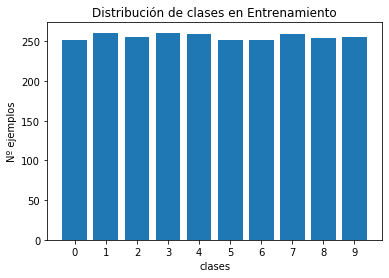
\includegraphics[scale=0.4]{imagenes/1.png}}
 \subfloat[]{
  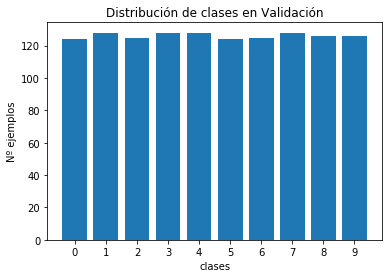
\includegraphics[scale=0.4]{imagenes/2.png}}
 \subfloat[]{
  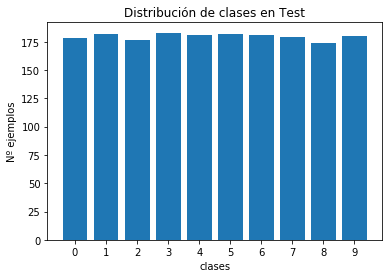
\includegraphics[scale=0.4]{imagenes/3.png}}
\end{figure}

El porcentaje de datos en cada conjunto es el siguiente:\\

Porcentaje de datos en entrenamiento (\%):  45.569395017793596

Porcentaje de datos en validación (\%):  22.455516014234874

Porcentaje de datos en test (\%):  31.97508896797153

\subsection{Regresión}

En el problema de regresión todos los datos vienen en un mismo fichero, así vamos a hacer una división de los datos de manera que un 50\% sea para training, un 25\% para validación y un 25\% para test.\\

En el código para separar los datos de training, validación y test hacemos uso de la función 
train\_test\_split de sklearn.model\_selection de la siguiente forma:

\begin{lstlisting}[frame=single]
        
x_train_original, x_test,  y_train_original, y_test = 
train_test_split(datos_x, datos_y, test_size=0.25)

x_train, x_val, y_train, y_val = train_test_split(x_train_original,
		 y_train_original, test_size=0.33)

\end{lstlisting}

Tras esta separación, el porcentaje de datos en cada conjunto es el siguiente:\\

Porcentaje de datos en entrenamiento (\%):  50.20060180541625

Porcentaje de datos en validación (\%):  24.77432296890672

Porcentaje de datos en test (\%):  25.025075225677032

\clearpage

\section{Preprocesado de datos}

En el preprocesado vamos a someter los datos de entrenamiento a varias transformaciones para luego facilitar su aprendizaje. Para encadenar las distintas transformaciones vamos a hacer uso de Pipeline de sklearn.pipeline.

\subsection{Clasificación}

En el problema de clasificación el preprocesado es el siguiente:

\begin{enumerate}
	\item Primero estandarizamos las características de forma que tengan media 0 y varianza unidad. Para ello hemos usado el método StandardScaler() de sklearn.preprocessing.
	\item Eliminamos las características cuya varianza sea muy pequeña, hemos puesto menor que 0.05, así eliminamos aquellas características que son constantes (no aportan nada) y las que varían muy poco. Hemos usado el método VarianceThreshold() de sklearn.feature\_selection pasándole como parámetro de umbral 0.05
	\item Generamos una nueva matriz de características consistente en las combinaciones polinomiales de las características que tenemos con grado menor o igual que 2. Para ello usamos PolynomialFeatures() de sklearn.preprocessing pasándole como parámetros degree=2 e interaction\_only=True. Al usar esos parámetros las nuevas características que obtengamos serán producto de características distintas (no se hace $x[1]^2$, $x[2]^2$, etc). Así conseguimos darle un mayor peso a la relación entre los bloques de píxeles a la hora de clasificar.
	\item Volvemos a estandarizar las características mediante el método StandardScaler(), hacemos ésto porque tras el paso anterior hemos modificado la varianza.
	\item Vamos a reducir la dimensionalidad usando análisis de componentes principales (PCA). Realizamos este paso porque tras usar PolynomialFeatures() hemos aumentado enormemente la dimensionalidad del problema. 
	
	Así, empleamos el método PCA() de sklearn.decomposition con el parámetro n\_components = 0.95, de forma que nos quedamos con el número de componentes que explican como mínimo el 95\% de la varianza.
	\item Volvemos a estandarizar las características mediante el método StandardScaler(), porque tras usar PCA hemos modificado la varianza.
\end{enumerate}

Comprobamos que el preprocesamiento ha surgido efecto mostrando los siguientes valores y gráficas.

\begin{table}[H]
\begin{tabular}{c|c|c|}
\cline{2-3}
                                                  & \textbf{Antes del preprocesamiento} & \textbf{Después del preprocesamiento} \\ \hline
\multicolumn{1}{|c|}{\textbf{Media}}              & 4.925291634127294                   & -1.4761127924892146e-18               \\ \hline
\multicolumn{1}{|c|}{\textbf{Varianza}}           & 6.03769649927445                    & 0.9999999999999997                    \\ \hline
\multicolumn{1}{|c|}{\textbf{Nº Características}} & 64                                  & 359                                   \\ \hline
\end{tabular}
\end{table}

\begin{figure}[H]
\centering
 \subfloat[Matriz de correlación antes del preprocesado]{
  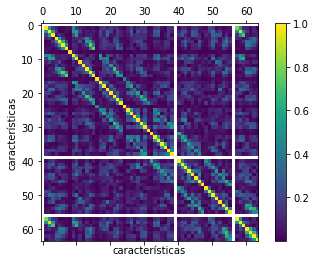
\includegraphics[scale=0.7]{imagenes/4.png}}
 \subfloat[Matriz de correlación después del preprocesado]{
  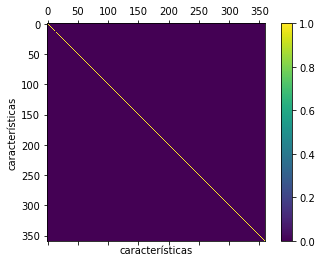
\includegraphics[scale=0.7]{imagenes/5.png}}
\end{figure}

\subsection{Regresión}

Es importante tener en cuenta que las 5 primeras características de los datos son no predictivas, es decir, no nos sirven para predecir el valor objetivo. Así que al leer los datos del fichero directamente eliminamos las 5 primeras columnas, que corresponden a dichas características.\\

En el problema de regresión el preprocesado es el siguiente:
\begin{enumerate}
	\item Primero completamos los datos, porque hay varios valores que faltan, así que cambiamos dichos valores desconocidos por la mediana de los valores de la característica correspondiente. Para ello hemos usado el método SimpleImputer() de sklearn.impute y le pasamos como argumento missing\_values=np.nan y strategy='median'.
	\item Estandarizamos las características de forma que tengan media 0 y varianza unidad. Para ello hemos usado el método StandardScaler() de sklearn.preprocessing.
\end{enumerate}

Comprobamos que el preprocesamiento ha surgido efecto mostrando los siguientes valores.

\begin{table}[H]
\begin{tabular}{c|c|c|}
\cline{2-3}
                                                  & \textbf{Antes del preprocesamiento} & \textbf{Después del preprocesamiento} \\ \hline
\multicolumn{1}{|c|}{\textbf{Media}}              & nan                  & -1.6379685148555003e-15               \\ \hline
\multicolumn{1}{|c|}{\textbf{Varianza}}           & nan                   & 1.0                    \\ \hline
\end{tabular}
\end{table}

Los valores nan en la media y la varianza antes del preprocesado se deben precisamente a los valores desconocidos.

\section{Elección de métrica a usar y discusión de su idoneidad}

\subsection{Clasificación}

En el problema de clasificación utilizamos como métrica Accuracy, ya que es una buena medida cuando las clases de variables de destino en los datos están casi equilibradas, que es precisamente nuestro caso como hemos visto anteriormente.\\

Con esta métrica calculamos $\frac{\text{nº etiquetas bien clasificadas}}{\text{nº etiquetas totales}}$
, dando como resultado un valor en el intervalor $[0,1]$, siendo $1$ el mejor resultado posible y $0$ el peor.\\

Se trata de una métrica simple pero idónea a nuestra problema gracias a la distribución de las clases.

\subsection{Regresión}

En el problema de regresión para ajustar los modelos usamos como métrica $\text{R}^2$, el coeficiente de determinación. Representa la proporción de la varianza (de las etiquetas) que ha sido explicada opr la variables independientes en el modelo.\\

Sea $\hat{y}_i$ el valor predicho por la muestra i-ésima e $y_i$ la correspondiente etiqueta real para un total de $n$ muestras, entonces $\text{R}^2$ se calcula como:

$$R^2(y, \hat{y}) = 1 - \frac{\sum_{i=1}^{n} (y_i - \hat{y}_i)^2}{\sum_{i=1}^{n} (y_i - \bar{y})^2} $$

La puntuación obtenida pertenece al intervalo $(- \infty, 1]$, donde $1$ es la mejor puntuación posible.\\

Utilizamos esta métrica porque proporciona una buena indicación de la bondad del ajuste y así una medida de la probabilidad de que nuevas muestras sean predicha por el modelo.

\section{Técnica de ajuste}

\subsection{Clasificación}

En el problema de clasificación la técnica de ajuste que utilizamos es una variación de SGD llamada SAG (Stochastic Average Gradient) en los modelos de RidgeClassifier y LogisticRegression de sklearn.linear\_model. \\

En el modelo RidgeClassifier minimizamos una suma de los cuadrados residual y penalizada: $\min_w ||Xw - y||_2^2 + \alpha||w||_2^2 $. Mientras que en el modelo LogisticRegression, tras la regularización, minimizamos la función:
$$\min_{2,c}\frac{1}{2}w^tw + C\sum_{i=1}^{n}\log(\exp(-y_i(X_i^Tw+c))+1)$$.\\

También usamos un modelo clasificador con SGD (SGDClassifier) en el que ajustamos mediante la función de pérdida 'hinge', de forma que minimizamos $\max(0,1-y_if(x_i))$, a lo que luego se le añade un sumando adicional por la regularización.\\

Se ha elegido la técnica de ajuste SAG porque garantiza una convergencia rápida cuando las características tienen aproximadamente la misma escala, lo cual ocurre en nuestro caso ya que todas las características comparten la misma escala.

\subsection{Regresión}

En el problema de regresión vamos a emplear dos modelos de sklearn.linear\_model que realizan ajustes distintos. En el primer modelo de regresión lineal, Lasso, ajustamos los coeficientes para minimizar la función $\min_{w} { \frac{1}{2N} ||X w - y||_2 ^ 2 + \alpha ||w||_1} $.\\

En el segundo modelo, SGDRegressor, ajustamos mediante la técnica SGD la función de pérdida de mínimos cuadrados ordinarios, de forma que minimizamos $||Xw - y||_2^2$, a lo que luego se le añade un sumando adicional por la regularización. 

Se ha elegido esta función de pérdida en el ajuste del modelo SGDRegressor, porque es la que se utiliza en sklearn por defecto y no se ha visto ninguna razón de peso para cambiarla en este caso.

\section{Regularización}

Tanto en el problema de clasificación como en el de regresión, debido a la gran complejidad que hay, es conveniente emplear una regularización para simplificar los modelos y que tengamos una generalización mejor.

\subsection{Clasificación}

En el problema de clasificación se ha utilizado la regularización l2 (Regularización Ridge), ya que seguramente la mayoría de los atributos de entrada son relevantes porque determinan el número de píxeles por bloque de la imagen y la mayor parte de esos bloques son esenciales a la hora de identificar el dígito.\\

Al aplicar esta regularización estamos añadiendo a la función del error un término nuevo, un sumando $\alpha ||w||_2^2$, siendo $\alpha$ un número real positivo. Así, con esta regularización hacemos que los coeficientes terminen siendo más pequeños, lo que minimiza el efecto de la correlación entre los atributos de entrada y hace que el modelo generalice mejor.

\subsection{Regresión}

En el problema de regresión estamos trabajando con un gran cantidad de características muy diversas y es muy probable que varias de ellas no influyan mucho en el modelo. Por ello, vamos a emplear una regularización l1 (Regularización Lasso).\\

Al aplicar esta regularización estamos añadiendo a la función del error un término nuevo, un sumando $\alpha ||w||_1$, siendo $\alpha$ un número real positivo. Así, con esta regularización hacemos que ciertos coeficientes tiendan a $0$.

\section{Definición de los modelos a usar}

En esta práctica estamos ajustando modelos lineales, por lo que todos los modelos que vamos a usar serán lineales. La implementación de los modelos utilizados proviene de  sklearn.linear\_model. 

\subsection{Clasificación}

En el problema de la clasificación los modelos que vamos a usar son los siguientes:

\begin{itemize}
	\item RidgeClassifier, se trata de un clasificador de regresión lineal al que se le impone una penalización en el tamaño de los coeficientes, dicha penalización es la regularización l2. Minimiza una suma de los cuadrados residual y penalizada: $\min_w ||Xw - y||_2^2 + \alpha||w||_2^2 $.
	\item LogisticRegression, es un modelo de clasificación lineal mediante regresión logística. Al aplicarse una regularización l2 minimiza la siguiente función: $$\min_{w, c} \frac{1}{2}w^T w + C \sum_{i=1}^n \log(\exp(- y_i (X_i^T w + c)) + 1)$$
	\item SGDClassifier, este estimador implementa un modelo lineal regularizado con aprendizaje mediante SGD. 
\end{itemize}

Otro modelo que se podría haber usado es el de Perceptron, pero se ha decidido no utilizarlo porque ya usamos SGDClassifier y Perceptron de sklearn.lineal\_model comparte la misma implementación subyacente con SGDClassifier.

\subsection{Regresión}

En el problema de regresión los modelos que vamos a usar son los siguientes:

\begin{itemize}
	\item Lasso, se trata de un modelo de regresión lineal al que se le impone una regularización l2 al entrenar. El objetivo de minimización para Lasso es: $\min_{w} { \frac{1}{2N} ||X w - y||_2 ^ 2 + \alpha ||w||_1} $, donde $N$ es el número de muestras.
	\item SGDRegressor, este regresor implementa un modelo lineal ajustado por una minimización de pérdida empírica con aprendizaje mediante SGD. 
\end{itemize}

\section{Estimación de los hiperparámetros y selección del mejor modelo}

\subsection{Clasificación}

Los hiperparámetros que hemos utilizado para las clasificaciones de los modelos son los siguientes:

-- En RidgeClasiffier:
\begin{itemize}
		\item solver='sag' para emplear Gradiente Estocástico Promedio descendente en las rutinas computacionales. Este solucionador garantiza una convergencia rápida cuando las características tienen aproximadamente la misma escala, lo cual ocurre en nuestro caso.
        \item max\_iter=500, ponemos el mismo número máximo de iteraciones en los tres modelos de clasificación para poder compararlos mejor y le asignamos 500 para que realice las suficientes iteraciones para converger.
\end{itemize}

-- En LogisticRegression:
\begin{itemize}
		\item penalty='l2' para emplear regularización l2
        \item solver='sag' para emplear Gradiente Estocástico Promedio descendente como algoritmo a usar en el problema de optimización.
        \item max\_iter=500, misma razón que antes, poder comparar mejor los modelos y permitir convergencia.
        \item multi\_class='multinomial', para que la pérdida minimizada sea la función de pérdida multinomial. En scikit-learn se sugiere utilizar 'multinomial' en el caso en que los datos no sean binarios ni se use solver='liblinear', que es precisamente nuestra situación.
\end{itemize}

-- En SGDClassifier:
\begin{itemize}
		\item loss = 'hinge', así la función de pérdida que se utiliza proporciona un SVM lineal. Es la función de pérdida por defecto y no se ha escogido otra porque con la regularización que empleamos si usamos loss='log' o loss='squared\_loss', entonces tendríamos regresión lógistica o clasificador Ridge respectivamente, los cuales ya hemos usado por lo que es preferible seguir con loss='hinge'.
        \item penalty = 'l2' para emplear regularización l2.
        \item max\_iter=500, misma razón que antes, poder comparar mejor los modelos y permitir convergencia.
\end{itemize}

El resto de hiperparámetros son los que se utilizan por defecto en dichos modelos de sklearn.linear\_model. \\

Los modelos se componen del preprocesado + clasificación y utilizamos Pipeline de sklearn.pipeline para componerlos. Los entrenamos haciendo uso del método fit de Pipeline y usando los datos de entrenamiento.\\

Para elegir el mejor modelo usamos la métrica de Accuracy discutida anteriormente para obtener el porcentaje de etiquetas predichas correctamente en el conjunto de validación. Seleccionaremos como mejor modelo aquel que mejor puntuación haya obtenido, en este caso ha sido el que tenía LogisticRegression como clasificador con los hiperparámetros ya mencionados.

Los resultados de las puntuaciones son los siguientes:

\begin{table}[H]
\centering
\begin{tabular}{c|c|c|}
\cline{2-3}
                                                      & \textbf{Accuracy en Training} & \textbf{Accuracy en Validación} \\ \hline
\multicolumn{1}{|c|}{\textbf{Regresíon lineal Ridge}} & 0.9945333853963295            & 0.9786053882725833              \\ \hline
\multicolumn{1}{|c|}{\textbf{Regresión Logística}}    & 1.0                           & 0.9817749603803486              \\ \hline
\multicolumn{1}{|c|}{\textbf{Clasificador SGD}}       & 0.9996095275283092            & 0.973851030110935               \\ \hline
\end{tabular}
\end{table}

\subsection{Regresión}

Los hiperparámetros que hemos utilizado para las regresiones de los modelos son los siguientes:

-- En Lasso:
\begin{itemize}
		\item alpha=0.0005, se trata de la constante que multiplica al término de regularización l1. Le hemos puesto un valor pequeño, pero distinto de $0$ (si ponemos alpha=0 no estamos usando la regularización), porque los valores pequeños para la regularización son los que mejores resultados nos han proporcionado en la práctica.
        \item max\_iter=1000, ponemos el mismo número máximo de iteraciones en los dos modelos de regresión para poder compararlos mejor y le asignamos 1000 para que realice las suficientes iteraciones para converger.
\end{itemize}

-- En SGDRegressor:
\begin{itemize}
		\item loss = 'squared\_loss', así la función de pérdida que se utiliza es la de mínimos cuadrados ordinarios.
        \item penalty = 'l1' para emplear regularización l1.
        \item max\_iter=1000, misma razón que antes, poder comparar mejor los modelos y permitir convergencia.
\end{itemize}

El resto de hiperparámetros son los que se utilizan por defecto en dichos modelos de sklearn.linear\_model. \\

Igual que en el problema de clasificación, los modelos se componen del preprocesado + clasificación y utilizamos Pipeline de sklearn.pipeline para componerlos. Los entrenamos haciendo uso del método fit de Pipeline y usando los datos de entrenamiento.\\

Para elegir el mejor modelo usamos la métrica $\text{R}^2$ discutida anteriormente para la puntuación de cada modelo. Seleccionaremos como mejor modelo aquel que mejor puntuación haya obtenido, en este caso ha sido el que tenía Lasso como regresor con los hiperparámetros ya mencionados.

Los resultados de las puntuaciones son los siguientes:

\begin{table}[H]
\centering
\begin{tabular}{c|c|c|}
\cline{2-3}
                                                      & \textbf{$\text{R}^2$ en Training} & \textbf{$\text{R}^2$ en Validación} \\ \hline
\multicolumn{1}{|c|}{\textbf{Lasso}} & 0.7120014138231237           & 0.6314331181491677             \\ \hline
\multicolumn{1}{|c|}{\textbf{SGDRegressor}}    & 0.6314331181491677                          & 0.6108542988770667             \\ \hline
\end{tabular}
\end{table}

\section{Estimación del error }

\subsection{Clasificación}

Una vez que tenemos seleccionado el modelo, volvemos a entrenarlo pero ésta vez usando el conjunto de train original, que es el compuesto por training+validación, y obtenemos el error tanto en training+validación como en test. 
Para obtener el error simplemente calculamos 1 - Accuracy, que es lo mismo que calcular $\frac{\text{número de etiquetas mal predichas}}{\text{número de etiquetas totales}}$.

\begin{table}[H]
\centering
\begin{tabular}{|l|l|}
\hline
\textbf{Error en training+validación}   & 0.0  \\ \hline
\textbf{Error en test} & 0.02114635503617135 \\ \hline
\end{tabular}
\end{table}

En la matriz de confusión que mostramos a continuación se pueden observar las predicciones realizadas en el conjunto de test:

\begin{figure}[H]
\centering
 \subfloat[]{
  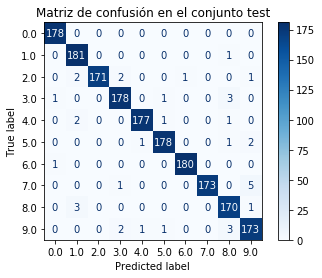
\includegraphics[scale=0.7]{imagenes/6.png}}
\end{figure}



Como el conjunto de los datos de test es totalmente independiente de los datos usados para el entrenamiento, porque todas las muestras y las personas que las han proporcionado son distintas, podemos usar el error en test como una estimación sin bias del error $E_{out}$.\\

Otra forma de estimar el error $E_{out}$ es mediante validación cruzada, de forma que usamos cross\_validate de sklearn.model\_selection para realizar $5$ particiones disjuntas del conjunto de entrenamiento y validación, usamos la media de los $5$ errores en validación para obtener una estimación del error $E_{out}$. Así obtenemos:

\begin{table}[H]
\centering
\begin{tabular}{|l|l|}
\hline
\textbf{Media de $E_{val}$ tras validación cruzada}   & 0.01647914314 \\ \hline
\end{tabular}
\end{table}

En nuestro caso, el error de $E_{test}$ es seguramente sea un mejor estimador de $E_{out}$ que la media de $E_{val}$, porque el valor de error es mayor y además el conjunto test es independiente del conjunto de entrenamiento.

\subsection{Regresión}

La métrica $\test{R}^2$ no nos proporciona directamente una medida del error. Así que además de mostrar las puntuaciones obtenidas con $\test{R}^2$ también vamos a mostrar el error RMSE, que nos proporciona la raíz del error cuadrático medio: $$\text{RMSE}(y, \hat{y}) = \sqrt{\frac{1}{N} \sum_{i=0}^{N - 1} (y_i - \hat{y}_i)^2}$$
donde $\hat{y}_i$ el valor predicho por la muestra i-ésima e $y_i$ la correspondiente etiqueta real para un total de $n$ muestras.\\

Una vez que hemos seleccionado el modelo, volvemos a entrenarlo pero ésta vez usando el conjunto compuesto por training+validación, y obtenemos el error tanto en training+validación como en test.

\begin{table}[H]
\centering
\begin{tabular}{c|c|c|}
\cline{2-3}
                                                & \textbf{Training+Validación} & \textbf{Test}       \\ \hline
\multicolumn{1}{|c|}{\textbf{R2}}               & 0.6949580455981569           & 0.6488809313269719  \\ \hline
\multicolumn{1}{|c|}{\textbf{RMSE}}             & 0.12945884098306587          & 0.13537712744998673 \\ \hline
\end{tabular}
\end{table}

Podemos usar el error en test como una estimación del error fuera de la muestra, ya que los datos de test no se han utilizado en ningún momento para ajustar el modelo.\\

Otra forma de estimar el error fuera de la muestra es mediante validación cruzada, de forma que volvemos a usar cross\_validate de sklearn.model\_selection para realizar $5$ particiones disjuntas del conjunto de entrenamiento y validación, usamos la media de los $5$ errores en validación para obtener una estimación del error $E_{out}$. 

Realizamos la validación cruzada usando la métrica de $\text{R}^2$ y RMSE, así obtenemos:

\begin{table}[H]
\centering
\begin{tabular}{|l|l|}
\hline
\textbf{Media de R2 tras validación cruzada}   & 0.6429521381408521  \\ \hline
\textbf{Media de RMSE tras validación cruzada} & 0.13889647897572635 \\ \hline
\end{tabular}
\end{table}

Como podemos observar, las dos estimaciones del error fuera de la muestra, que serían los valores de $\text{R}^2$ y RMSE obtenidos en el conjunto de test y la media tras validación cruzada, proprocionan valores muy similares. 

\clearpage

\section{Justificación del mejor modelo}

\subsection{Clasificación}

Teniendo en cuenta los valores de las puntuaciones, errores obtenidos y la matriz de confusión se puede observar que efectivamente el modelo seleccionado, el clasificador de regresión logística con los hiperparámetros especificados previamente, representa adecuadamente los datos con una calidad muy buena. \\

Si fuera el encargado de realizar este ajuste para una empresa les propondría el modelo mencionado.

Clasifica correctamente alrededor del 98\% de los dígitos del conjunto de test, por lo que es esperable que el error de $E_{out}$ que se vaya a cometer sea similar, sólamente alrededor de un 2\% de error. \\

El modelo es claramente el que mejor error proporciona de entre los que se han probado, ya que lo hemos escogido precisamente por ser el que mejor puntuación obtiene. Aun así, evidentemente no podemos asegurar que sea el mejor modelo que exista, pero sí que es un modelo con un error muy bajo y que clasifica bien con una precisión muy alta los dígitos. 

\subsection{Regresión}

Teniendo en cuenta los valores de las puntuaciones y errores obtenidos se puede observar que efectivamente el modelo seleccionado, el regresor lineal Lasso con los hiperparámetros especificados previamente predice los datos con una calidad aceptable. 

La estimación del coeficiente de determinación fuera de la muestra se sitúa sobre el 0.65, que está lejos del ajuste perfecto que sería 1, pero tampoco es un valor terrible, indica que el modelo explica más del 60\% de la varianza.\\

Fijándonos ahora en el error RMSE, su estimación fuera de la muestra se sitúa alrededor del 0.14. Otra vez, no es un valor excelente, pero indica que el error que se comete tampoco es muy grande. A partir de las características con las que estamos trabajando puede predecir el número de crímenes violentos per cápita comitiendo un fallo sobre $\pm 0.2$ en media con cierta seguridad.\\

El modelo es el que mejor error proporciona de entre los que se han probado, ya que lo hemos escogido precisamente por ser el que mejor puntuación obtiene. Aun así, evidentemente no podemos asegurar que sea el mejor modelo que exista, hay un margen de mejora para nada despreciable.

\end{document}